\section{$\rho_2$ cannot be a 4-transposition}

\paragraph{}
By Lemma~\ref{min-4-trans}, one of the $\rho_i$'s must be a 4-transposition. But we proved in Lemma~\ref{exclude-0} and~\ref{exclude-1} that there are no string C-group representation of $A_{11}$ if $\rho_0$, $\rho_1$, $\rho_3$ or $\rho_4$ are 4-transpositions.

\paragraph{}
In Lemma~\ref{find-2} we use the Method~\ref{method} to find some sggis. The permutation representation graphs of those sggis are displayed in appendix~\ref{monodromy-5}. After that we prove in Lemma~\ref{exclude-2} that none of those sggis satisfy the intersection property and thus none of them are string C-groups.

\begin{lemma}
  \label{find-2}
  Suppose that $\rho_2$ is a 4-transposition, all sggis of rank 5 that generates $A_{11}$ are those displayed in appendix~\ref{monodromy-5} (p.~\pageref{monodromy-5}).
\end{lemma}

\begin{proof}
  In this case, we start with the $\rho_2$ 4-transposition.

  \begin{figure}[H]
    \begin{center}
      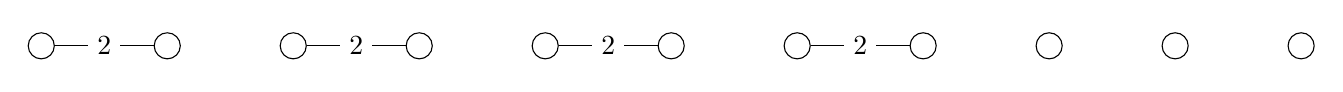
\begin{tikzpicture}[scale=.8]

        \begin{scope}[every node/.style={circle,draw}]
          \node (1)  at (-2,0)  {};
          \node (2)  at (0,0)  {};
          \node (3)  at (2,0)  {};
          \node (4)  at (4,0)  {};
          \node (5)  at (6,0)  {};
          \node (6)  at (8,0)  {};
          \node (7)  at (10,0)  {};
          \node (8)  at (12,0)  {};
          \node (9)  at (14,0)  {};
          \node (10)  at (16,0)  {};
          \node (11)  at (18,0)  {};
        \end{scope}

        \begin{scope}[every node/.style={fill=white}]

          \begin{scope}[every edge/.style={draw}]
            \path (1)  edge node {$2$} (2);
            \path (3)  edge node {$2$} (4);
            \path (5)  edge node {$2$} (6);
            \path (7)  edge node {$2$} (8);
          \end{scope}
        \end{scope}

      \end{tikzpicture}
      \caption{}
    \end{center}
  \end{figure}

\paragraph{}
The involutions $\rho_0$ and $\rho_4$ must commute with $\rho_2$ thus when adding their edges to the graph, only the patterns seen in Proposition~\ref{patterns-adding} are possible. But $\rho_0$ and $\rho_4$ must commute too. Thus they must form patterns saw in Proposition~\ref{intersection-patterns}.

\paragraph{}
Since there is only one 4-transposition, there are only 12 edges available to link 11 points, 2 more than the minimum. Thus if an edge is added, it must link two distinct components, except two times. Those two edges are called "joker" edges. When an alternating square is built, one of those edges is used, it is the same if a double edge is built.

\paragraph{}
A choice must be made among the three possibilities for each involution. We prove that one involution must form an alternating square and that the other must make a double edge and link two fixed points of $\rho_2$.

\paragraph{}
First, we prove that none of the involutions can make two double edges. We then prove that both involutions cannot make the same pattern i.e. both involutions cannot make an alternate square and both involutions cannot make a double edge.

\paragraph{}
Each pattern of Lemma~\ref{patterns-adding} uses at least one "joker" edge. Thus none of the patterns that we use can use both "joker" edges and leave nothing to the other involution. Therefore the pattern consisting of two double edges is impossible.

\paragraph{}
Now we prove that both patterns cannot build one double edge and link two fixed points at the same time. There are only three points fixed by $\rho_2$. If both involutions make one double edge and link two fixed points they must share at least one of the fixed points. Therefore a $\rho_0$ and a $\rho_4$ edge share a vertex but that is forbidden by Lemma~\ref{0-4-no-share}.

\paragraph{}
If both involutions make an alternating square with $\rho_2$ there are two possibilities: the two squares can share some vertices or none.


\paragraph{}
If they share some vertices then a $\rho_0$ and a $\rho_4$ involution share a vertex but that is forbidden by Lemma~\ref{0-4-no-share}.

\paragraph{}
If the two squares do not share a vertex, the graph is the following.

\begin{figure}[H]
  \begin{center}
    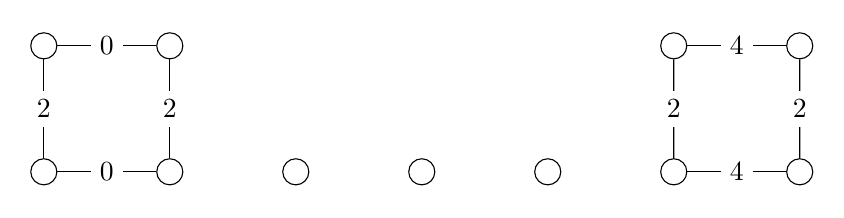
\begin{tikzpicture}[scale=.8]

      \begin{scope}[every node/.style={circle,draw}]
        \node (1)  at (0,0)  {};
        \node (2)  at (0,2)  {};
        \node (3)  at (2,0)  {};
        \node (4)  at (2,2)  {};
        \node (5)  at (4,0)  {};
        \node (6)  at (6,0)  {};
        \node (7)  at (8,0)  {};
        \node (8)  at (10,0)  {};
        \node (9)  at (10,2)  {};
        \node (10)  at (12,0)  {};
        \node (11)  at (12,2)  {};
      \end{scope}

      \begin{scope}[every node/.style={fill=white}]

        \begin{scope}[every edge/.style={draw}]
          \path (1)  edge node {$0$} (3);
          \path (2)  edge node {$0$} (4);
          \path (1)  edge node {$2$} (2);
          \path (3)  edge node {$2$} (4);
          \path (8)  edge node {$2$} (9);
          \path (10) edge node {$2$} (11);
          \path (8)  edge node {$4$} (10);
          \path (9)  edge node {$4$} (11);
        \end{scope}
      \end{scope}

    \end{tikzpicture}
    \caption{}
  \end{center}
\end{figure}

\paragraph{}
All "joker" edges have been used so no more alternating square can be built. But the left square must be connected by a $\rho_1$ edge and the right one by a $\rho_3$ edge by Proposition~\ref{square-connection}. We need to find a chain that connects the left square to the right square with only $\rho_1$ and $\rho_3$ edges. But that is impossible because the indices must be consecutive in a chain by Lemma~\ref{chain-consecutive}.

\paragraph{}
In summary, because the pattern with two double edges cannot be used and because the same pattern cannot be used twice, one of the involution must build an alternating square and the other must build a double edge and link two fixed points. By duality, we only consider the case where $\rho_4$ makes an alternating square. Thus $\rho_0$ makes a double edge and links two fixed points of $\rho_4$.

\begin{figure}[H]
  \begin{center}
    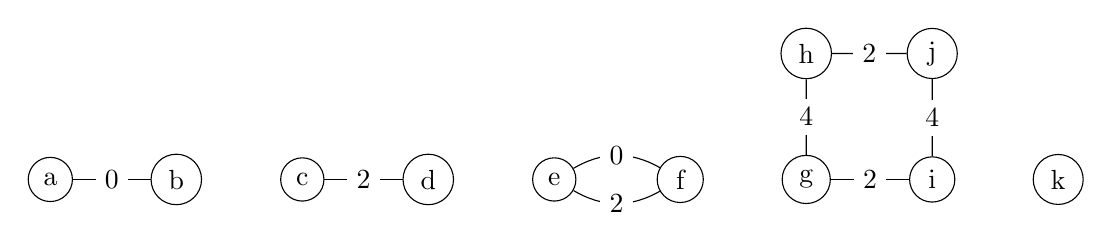
\begin{tikzpicture}[scale=.8]

      \begin{scope}[every node/.style={circle,draw}]
        \node (1)  at (12,2)  {h};
        \node (2)  at (12,0)  {g};
        \node (3)  at (14,2)  {j};
        \node (4)  at (14,0)  {i};
        \node (5)  at (6,0)  {d};
        \node (6)  at (4,0)  {c};
        \node (7)  at (10,0)  {f};
        \node (8)  at (8,0)  {e};
        \node (9)  at (2,0)  {b};
        \node (10) at (0,0)  {a};
        \node (11) at (16,0) {k};
      \end{scope}

      \begin{scope}[every node/.style={fill=white}]

        \begin{scope}[every edge/.style={draw}]
          \path (9)  edge node {$0$} (10);
          \path (7)  edge[bend right=30] node {$0$} (8);
          \path (1)  edge node {$2$} (3);
          \path (2)  edge node {$2$} (4);
          \path (5)  edge node {$2$} (6);
          \path (7)  edge[bend left=30] node {$2$} (8);
          \path (1)  edge node {$4$} (2);
          \path (3)  edge node {$4$} (4);
        \end{scope}
      \end{scope}

    \end{tikzpicture}
    \caption{The graph with $\rho_0$, $\rho_2$ and $\rho_4$}
  \end{center}
\end{figure}

\paragraph{}
All of our "joker" edges have been used, every other unplaced edge must thus link two different connected components of the graph.

\paragraph{}
Now the $\rho_3$ edge is placed. It cannot be adjacent to the component $\{a,b\}$ and $\{e,f\}$ by Proposition~\ref{chain-consecutive} and~\ref{adjacent-double} respectively. There are three components that can be connected by two $\rho_3$ edges. After placing all $\rho_3$ edges, those three components form one big component. The $\rho_1$ edges are then placed and they must connect to this new component. The edge $(c,d)$ is the only component among the three that can be connected to a $\rho_1$ edge. Therefore one end of this edge must remain free.

\paragraph{}
The fixed point cannot be connected twice by $\rho_3$ edges by Proposition~\ref{fixed-only-1}. So there is only one possibility. One edge must connect the component $\{e,f\}$ to the component $\{g,h,i,j\}$ and the other must connect $\{g,h,i,j\}$ to the fixed point $k$.

\paragraph{}
Now we have multiple cases depending on the vertices chosen on the square. In fact, no other edge will be connected to the square later in this proof. Thus we only consider one of the three cases in the following statements.

\paragraph{}
The three cases are: two opposed vertices on the square, two adjacent vertices in the square, separated by either $\rho_1$ or $\rho_3$. Those cases generate three different graphs, only one is kept in the proof. The reader can look at Appendix~\ref{monodromy-5} for the other possibilities.

\begin{figure}[H]
  \begin{center}
    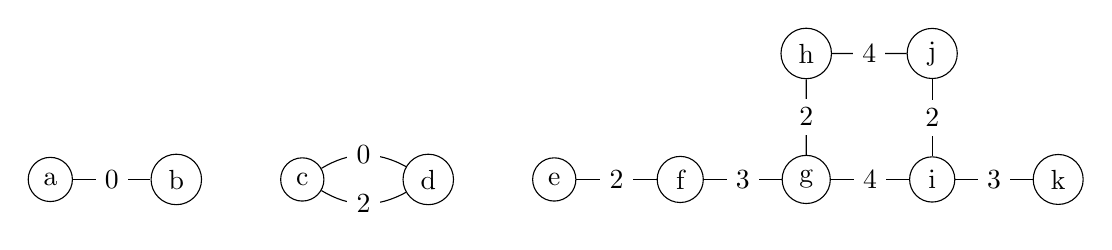
\begin{tikzpicture}[scale=.8]

      \begin{scope}[every node/.style={circle,draw}]
        \node (1)  at (0,2)  {j};
        \node (2)  at (0,0)  {i};
        \node (3)  at (-2,2)  {h};
        \node (4)  at (-2,0)  {g};
        \node (5)  at (-6,0)  {e};
        \node (6)  at (-4,0)  {f};
        \node (7)  at (-10,0)  {c};
        \node (8)  at (-8,0)  {d};
        \node (9)  at (-14,0)  {a};
        \node (10) at (-12,0)  {b};
        \node (11) at (2,0) {k};
      \end{scope}

      \begin{scope}[every node/.style={fill=white}]

        \begin{scope}[every edge/.style={draw}]
          \path (9)  edge node {$0$} (10);
          \path (7)  edge[bend left=30] node {$0$} (8);
          \path (1)  edge node {$2$} (2);
          \path (3)  edge node {$2$} (4);
          \path (5)  edge node {$2$} (6);
          \path (7)  edge[bend right=30] node {$2$} (8);
          \path (2)  edge node {$3$} (11);
          \path (4)  edge node {$3$} (6);
          \path (1)  edge node {$4$} (3);
          \path (2)  edge node {$4$} (4);
        \end{scope}
      \end{scope}

    \end{tikzpicture}
    \caption{One of the graphs after placing $\rho_3$ edges}
  \end{center}
\end{figure}

\paragraph{}
Now the two edges of $\rho_1$ must be placed. A $\rho_1$ edge must link the component $\{a,b\}$ and $\{c,d\}$. Due to the symmetry, the choice of the points does not change anything. We choose to link $b$ and $c$.

\begin{figure}[H]
  \begin{center}
    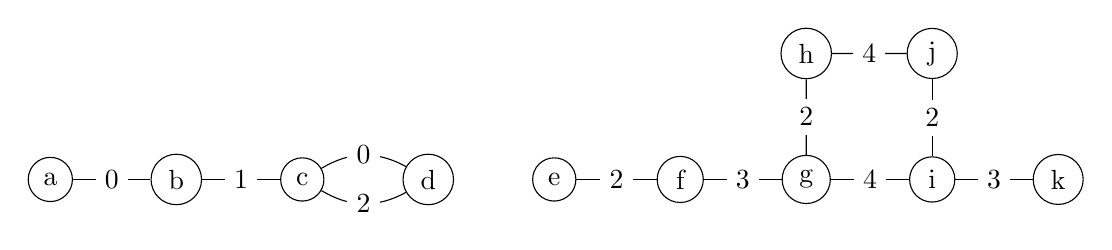
\begin{tikzpicture}[scale=.8]

      \begin{scope}[every node/.style={circle,draw}]
        \node (1)  at (0,2)  {j};
        \node (2)  at (0,0)  {i};
        \node (3)  at (-2,2)  {h};
        \node (4)  at (-2,0)  {g};
        \node (5)  at (-6,0)  {e};
        \node (6)  at (-4,0)  {f};
        \node (7)  at (-10,0)  {c};
        \node (8)  at (-8,0)  {d};
        \node (9)  at (-14,0)  {a};
        \node (10) at (-12,0)  {b};
        \node (11) at (2,0) {k};
      \end{scope}

      \begin{scope}[every node/.style={fill=white}]

        \begin{scope}[every edge/.style={draw}]
          \path (9)  edge node {$0$} (10);
          \path (7)  edge[bend left=30] node {$0$} (8);
          \path (10) edge node {$1$} (7);
          \path (1)  edge node {$2$} (2);
          \path (3)  edge node {$2$} (4);
          \path (5)  edge node {$2$} (6);
          \path (7)  edge[bend right=30] node {$2$} (8);
          \path (2)  edge node {$3$} (11);
          \path (4)  edge node {$3$} (6);
          \path (1)  edge node {$4$} (3);
          \path (2)  edge node {$4$} (4);
        \end{scope}
      \end{scope}

    \end{tikzpicture}
    \caption{}
  \end{center}
\end{figure}


\paragraph{}
The component $\{e,f,g,h,i,j,k\}$ must be linked by $e$ as explained above. For the component $\{a,b,c,d\}$ there are two possibilities: $a$ or $d$. Both solutions create a valid sggi graph. Here is one of the graphs:

\begin{figure}[H]
  \begin{center}
    \begin{tikzpicture}[scale=.8]

      \begin{scope}[every node/.style={circle,draw}]
        \node (1)  at (0,2)  {};
        \node (2)  at (0,0)  {};
        \node (3)  at (-2,2)  {};
        \node (4)  at (-2,0)  {};
        \node (5)  at (-6,0)  {};
        \node (6)  at (-4,0)  {};
        \node (7)  at (-10,0)  {};
        \node (8)  at (-8,0)  {};
        \node (9)  at (-14,0)  {};
        \node (10) at (-12,0)  {};
        \node (11) at (2,0) {};
      \end{scope}

      \begin{scope}[every node/.style={fill=white}]

        \begin{scope}[every edge/.style={draw}]
          \path (9)  edge node {$0$} (10);
          \path (7)  edge[bend left=30] node {$0$} (8);
          \path (5)  edge node {$1$} (8);
          \path (7)  edge node {$1$} (10);
          \path (1)  edge node {$2$} (2);
          \path (3)  edge node {$2$} (4);
          \path (5)  edge node {$2$} (6);
          \path (7)  edge[bend right=30] node {$2$} (8);
          \path (2)  edge node {$3$} (11);
          \path (4)  edge node {$3$} (6);
          \path (1)  edge node {$4$} (3);
          \path (2)  edge node {$4$} (4);
        \end{scope}
      \end{scope}

    \end{tikzpicture}
    \caption{One sggi on $A_{11}$ of rank 5}
  \end{center}
\end{figure}

\paragraph{}
When placing the $\rho_3$ edge we made a choice among three possibilities, for the $\rho_1$ edge it was among two possibilities. Thus in total there are 6 graphs. The construction of the five other graphs is left to the reader. He can check that the built graphs match the graphs of appendix~\ref{monodromy-5}.

\end{proof}


\begin{lemma}
  \label{exclude-2}
  None of the six sggis represented by the graphs of appendix~\ref{monodromy-5} are string C-groups representation of $A_{11}$.
\end{lemma}

\begin{proof}
  By the definition of a C-group, it is sufficient to find two subsets of generators $S_1$ and $S_2$ such that $\Gamma_{S_1} \cap \Gamma_{S_2} \neq \Gamma_{S_1 \cap S_2}$.

  \paragraph{}
  This proof is inspired by section 4 of~\cite{leemansTransactions}.

  \paragraph{}
  In this case, we choose $S_1 = \{\rho_1, \rho_2\}$ and $S_2 = \{\rho_2, \rho_3, \rho_4\}$. Here $S_1 \cap S_2 = \{\rho_2\}$ and so $\Gamma_{S_1 \cap S_2} = \Gamma_{\rho_2}$ is a cyclic group of order 2. Hence, $\rho_2$ is an involution.

  \paragraph{}
  $S_1$ is studied more deeply. Only the $\rho_1$ and $\rho_2$ edges are kept in all the possible graphs. There are only two possible graphs:

  \begin{figure}[H]
    \begin{center}
      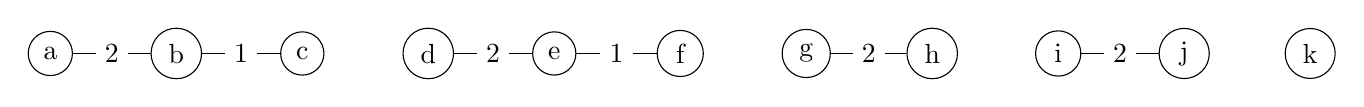
\begin{tikzpicture}[scale=.8]

        \begin{scope}[every node/.style={circle,draw}]
          \node (1)  at (-2,0)  {a};
          \node (2)  at (0,0)  {b};
          \node (3)  at (2,0)  {c};
          \node (4)  at (8,0)  {f};
          \node (5)  at (6,0)  {e};
          \node (6)  at (4,0)  {d};
          \node (7)  at (12,0)  {h};
          \node (8)  at (10,0)  {g};
          \node (9)  at (16,0)  {j};
          \node (10) at (14,0)  {i};
          \node (11)  at (18,0)  {k};
        \end{scope}

        \begin{scope}[every node/.style={fill=white}]

          \begin{scope}[every edge/.style={draw}]
            \path (2)  edge node {$1$} (3);
            \path (4)  edge node {$1$} (5);
            \path (1)  edge node {$2$} (2);
            \path (5)  edge node {$2$} (6);
            \path (7)  edge node {$2$} (8);
            \path (9)  edge node {$2$} (10);
          \end{scope}
        \end{scope}

      \end{tikzpicture}
      \caption{First possibility for $\Gamma_{S_1}$}
    \end{center}
  \end{figure}

  \begin{figure}[H]
    \begin{center}
      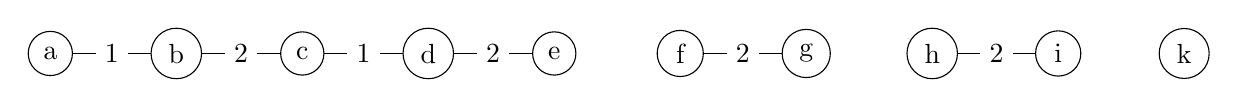
\begin{tikzpicture}[scale=.8]

        \begin{scope}[every node/.style={circle,draw}]
          \node (2)  at (0,0)  {a};
          \node (3)  at (2,0)  {b};
          \node (4)  at (4,0)  {c};
          \node (5)  at (6,0)  {d};
          \node (6)  at (8,0)  {e};
          \node (7)  at (12,0)  {g};
          \node (8)  at (10,0)  {f};
          \node (9)  at (16,0)  {i};
          \node (10) at (14,0)  {h};
          \node (1)  at (18,0)  {k};
        \end{scope}

        \begin{scope}[every node/.style={fill=white}]

          \begin{scope}[every edge/.style={draw}]
            \path (2)  edge node {$1$} (3);
            \path (4)  edge node {$1$} (5);
            \path (3)  edge node {$2$} (4);
            \path (5)  edge node {$2$} (6);
            \path (7)  edge node {$2$} (8);
            \path (9)  edge node {$2$} (10);
          \end{scope}
        \end{scope}

      \end{tikzpicture}
      \caption{Second possibility for $\Gamma_{S_1}$}
    \end{center}
  \end{figure}

  \paragraph{}
  In the first graph, the permutation $(\rho_1 \rho_2)^2 \rho_1$ is $(a~b)(d~e)$. Thus this permutation permutes only 4 out of the 8 points of $\rho_2$.

  \paragraph{}
  In the second graph, $(\rho_1\rho_2)^4 \rho_1 = (b~c)(d~e)$ gives the same result.

  \paragraph{}
  With $S_2$, the disposition of the edges alongside the alternating square is very important. Therefore there are 3 possibilities among the six graphs:

  \begin{figure}[H]
    \begin{center}
      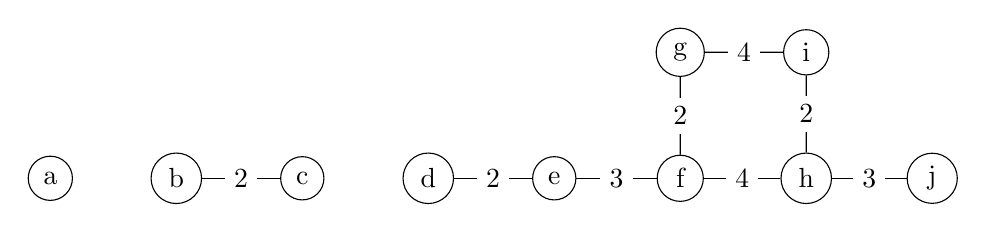
\begin{tikzpicture}[scale=.8]

        \begin{scope}[every node/.style={circle,draw}]
          \node (0)  at (-4,0)  {a};
          \node (1)  at (-2,0)  {b};
          \node (2)  at (0,0)  {c};
          \node (5)  at (2,0)  {d};
          \node (6)  at (4,0)  {e};
          \node (7)  at (6,0)  {f};
          \node (8)  at (6,2)  {g};
          \node (9)  at (8,2)  {i};
          \node (10) at (8,0)  {h};
          \node (11) at (10,0) {j};
        \end{scope}

        \begin{scope}[every node/.style={fill=white}]

          \begin{scope}[every edge/.style={draw}]
            \path (1)  edge node {$2$} (2);
            \path (5)  edge node {$2$} (6);
            \path (7)  edge node {$2$} (8);
            \path (9)  edge node {$2$} (10);
            \path (6)  edge node {$3$} (7);
            \path (10) edge node {$3$} (11);
            \path (7)  edge node {$4$} (10);
            \path (8)  edge node {$4$} (9);
          \end{scope}
        \end{scope}

      \end{tikzpicture}
      \caption{First possibility for $\Gamma_{S_2}$}
      \label{S2-1}
    \end{center}
  \end{figure}

  \begin{figure}[H]
    \begin{center}
      \begin{tikzpicture}[scale=.8]

        \begin{scope}[every node/.style={circle,draw}]
          \node (0)  at (-4,0)  {};
          \node (1)  at (-2,0)  {};
          \node (2)  at (0,0)  {};
          \node (5)  at (2,0)  {};
          \node (6)  at (4,0)  {};
          \node (7)  at (6,0)  {};
          \node (8)  at (6,2)  {};
          \node (9)  at (8,0)  {};
          \node (10) at (8,2)  {};
          \node (11) at (10,2) {};
        \end{scope}

        \begin{scope}[every node/.style={fill=white}]

          \begin{scope}[every edge/.style={draw}]
            \path (1)  edge node {$2$} (2);
            \path (5)  edge node {$2$} (6);
            \path (7)  edge node {$2$} (8);
            \path (9)  edge node {$2$} (10);
            \path (6)  edge node {$3$} (7);
            \path (10) edge node {$3$} (11);
            \path (7)  edge node {$4$} (9);
            \path (8)  edge node {$4$} (10);
          \end{scope}
        \end{scope}

      \end{tikzpicture}
      \caption{Second possibility for $\Gamma_{S_2}$}
    \end{center}
  \end{figure}

  \begin{figure}[H]
    \begin{center}
      \begin{tikzpicture}[scale=.8]

        \begin{scope}[every node/.style={circle,draw}]
          \node (0)  at (-4,0)  {};
          \node (1)  at (-2,0)  {};
          \node (2)  at (0,0)  {};
          \node (5)  at (2,0)  {};
          \node (6)  at (4,0)  {};
          \node (7)  at (8,2)  {};
          \node (8)  at (6,2)  {};
          \node (9)  at (6,0)  {};
          \node (10) at (8,0)  {};
          \node (11) at (10,0) {};
        \end{scope}

        \begin{scope}[every node/.style={fill=white}]

          \begin{scope}[every edge/.style={draw}]
            \path (1)  edge node {$2$} (2);
            \path (5)  edge node {$2$} (6);
            \path (7)  edge node {$2$} (8);
            \path (9)  edge node {$2$} (10);
            \path (6)  edge node {$3$} (9);
            \path (10) edge node {$3$} (11);
            \path (7)  edge node {$4$} (10);
            \path (8)  edge node {$4$} (9);
          \end{scope}
        \end{scope}

      \end{tikzpicture}
      \caption{Third possibility for $\Gamma_{S_2}$}
    \end{center}
  \end{figure}

  \paragraph{}
  We only do the graph displayed in Figure~\ref{S2-1}. The proof is similar for the two other graphs and is left to the reader.

  \paragraph{}
  We prove that $\Gamma_{\rho_2,\rho_3,\rho_4}$ is isomorphic to $S_7$ on the component $\{d,e,f,g,h,i,j\}$. For this purpose, we first prove that the group is 2-transitive. Thus by Property~\ref{2-transitive-primitive}, it is primitive. The primitive group are well-known and the list of all primitive groups of degree less than 50 is available in~\cite{buekenhout1996list}.

  \paragraph{}
  The group is transitive because its graph is connected. To prove that the group is 2-transitive we use Property~\ref{practical-transitivity}. We try to find a permutation that send $h$ to any other point while keeping $j$ fixed. If the permutation does not contain $\rho_3$ then $j$ is fixed. Thus in fact there are two orbits : $\{d,e\}$ and $\{f,g,h,i\}$. The vertex $h$ is already in the second orbit, thus it can be easily sent to every other point of the orbit.

  \paragraph{}
  We need to find a permutation that sends $h$ to $d$ or $e$ while keeping $j$ in place. The permutation $\rho_2 \rho_4 \rho_3 \rho_2 \rho_3 \rho_2 \rho_3$ is a solution that sends $h$ to $d$. $\Gamma_{\rho_2, \rho_3, \rho_4}$ is 2-transitive and thus primitive on $\{d,e,f,g,h,i,j\}$

  \paragraph{}
  We now look at the list of all primitive groups~\cite{buekenhout1996list}. We compute the size of some subgroups. By Property~\ref{magic-formula} the order of a group is a multiple of the size of its subgroups. Thus the order of the group must be an multiple of the least common multiple of the size of some subgroups.

  \paragraph{}
  The group is 2-transitive and so its order is a multiple of $7 \times 6 = 42$. $\Gamma_{\rho_2, \rho_3}$ is $D_{24}$ which is of order 24. Thus the order of the group must be a multiple of the least common divisor of 42 and 10 which is 168. But the only groups that satisfies this condition are $PSL_3(2)$, $A_7$ and $S_7$. But $D_{24}$ is not a subgroup of $\PSL_3(2)$. Moreover $\rho_2$ is an odd involution and cannot be member of $A_7$ thus the group generated by this graph must be $S_7$.

  \paragraph{}
  Then every $\rho_2$ edge becomes an involution on those seven points. Thus it is also possible to find a permutation that only moves 4 points out of the 8 points of $\rho_2$. This permutation is in $\Gamma_{S_1}$ and in $\Gamma_{S_2}$ but not in $\Gamma_{\rho_2}$ thus $\Gamma$ does not satisfy the intersection property and is not a C-group.

\end{proof}

\paragraph{}
now

\begin{theorem}
  There does not exist a string C-group representation of rank 5 of $A_{11}$.
\end{theorem}

\paragraph{}
Now we have proved that there is no abstract polytopes of rank $5$ on $A_{11}$. Next we prove the same for rank 4.
